\documentclass{beamer}
\usetheme{Madrid}



 % Algorithms
\usepackage{algorithm}
%\usepackage[noend]{algpseudocode}
\usepackage{algpseudocode}

% Macros for definitions
% Assumptions
\newcommand{\as}[1][]{\ensuremath{\mathcal{A}_{#1}}}
\newcommand{\asemt}{\as[\perp]}
\newcommand{\ain}{\mathcal{A}_{in}}
\newcommand{\ASphi}{\ensuremath{AS_{\kf{i}{}}^\varphi}}
\newcommand{\sem}{\ensuremath{\mathcal{C}_{\kf{i}{}}^\varphi}}

% Algorithm
\newcommand{\method}[1]{\textnormal{\textsc{#1}}}

%True, false
\newcommand{\true}{\ensuremath{\texttt{tt}}}
\newcommand{\false}{\ensuremath{\texttt{ff}}}

% Kripke
\newcommand{\ks}[1][]{\ensuremath{\mathcal{K}_{#1}}}
\newcommand{\kf}[2]{\ensuremath{\mathcal{F}^{#2}_{#1}}}
\newcommand{\fullKs}{\ensuremath{ \ks = (\params, S, S_0, \trans{}, L) }}
\newcommand{\fullKf}[2]{\ensuremath{ \kf{#1}{#2} = (\params, S_{#1}, I_{i}, \trans{}_{#1}, L_{#1}) }}
\newcommand{\trans}[1]{\stackrel{#1}{\rightarrow}}
\newcommand{\params}{\mathcal{P}}

%Temporal
\newcommand{\eu}[2]{\ensuremath{\mbox{E} #1 \mbox{U} #2 }}
\newcommand{\au}[2]{\ensuremath{\mbox{A} #1 \mbox{U} #2 }}
\newcommand{\ex}[1]{\ensuremath{\mbox{EX} #1}}
\newcommand{\ax}[1]{\ensuremath{\mbox{AX} #1}}
\newcommand{\ef}[1]{\ensuremath{\mbox{EF} #1}}
\newcommand{\af}[1]{\ensuremath{\mbox{AF} #1}}
\newcommand{\eg}[1]{\ensuremath{\mbox{EG} #1}}
\newcommand{\ag}[1]{\ensuremath{\mbox{AG} #1}}

 \algblockdefx{ForAllPar}{EndForPar}[2]%
 {\textbf{for all }#1 \textbf{do in parallel} #2}%


\usepackage{wrapfig}

\title[Scalable Parameter Synthesis] % (optional, only for long titles)
{Scalable Parameter Synthesis from CTL Hypotheses}
\author[Pastva] % (optional, for multiple authors)
{Samuel Pastva}
\institute[Masaryk University] % (optional)
{
	Masaryk University \\
	Brno
}
\date[2015] % (optional)
{Bachelor Thesis, 2015}
\subject{Computer Science}

\begin{document}
  \frame{\titlepage}
  \begin{frame}
    \frametitle{Goals}
		\begin{itemize}
			\item<1-> Design a distributed memory algorithm that computes the Parameter Synthesis Problem for biochemical models and CTL hypotheses, i.e. states and parameter values of investigated model where given hypothesis is satisfied.
			\item<2-> Implement the algorithm and integrate it with existing modelling frameworks for ODE models and Thomas Networks (Biodivine and Parsybone).
			\item<3-> Test and benchmark the algorithm on existing biochemical models.
		\end{itemize}
  \end{frame}
  \begin{frame}
    \frametitle{Why CTL?}
    Similar technique already exist for LTL - Why do we need CTL for biochemical models?
	\begin{itemize}
		\item<1-> Different expressive power than LTL		
				
			$CTL \not\subseteq LTL \wedge LTL \not\subseteq CTL$				
		\item<2-> We can test for properties that can't be expressed in LTL, such as multistability			  
		\item<3-> Globality - it is easier to obtain global information about whole model using CTL rather than LTL.
	\end{itemize}
  \end{frame}
  \begin{frame}
  	\frametitle{Model}
  	As an input to our algorithm, we consider Parametrised Kripke Structure:
  	\begin{block}{Parametrised Kripke Structure(PKS)}
  			$\fullKs$
			\begin{itemize}
				\item $\params$ is a finite set of parameters (all possible parameter valuations)
				\item $S$ is a finite set of states
				\item $S_0 \subseteq S$ is a set of initial states
				\item $\trans{} \subseteq S \times \params \times S$ is a transition relation labelled by parameter valuations 
				\item $L: S \rightarrow 2^{AP} $ is a labelling function from states to sets of atomic propositions which are true in such states
			\end{itemize}
	\end{block}
  \end{frame}
  \begin{frame}
  	\frametitle{State Space Distribution}
  	In order to distribute the computation across $N$ workstations, we use distribution function $f: S \rightarrow \{1, \dots, N\}$.
  	
  	The distribution function divides the original PKS into $N$ \emph{Kripke Fragments}. 
  	
  	Each fragment contains states described in distribution function plus all direct successors of these states (border states).
  	
  	Each border state represents a remaining portion of the state space located at another workstation.
  	
  	\begin{center}
	  	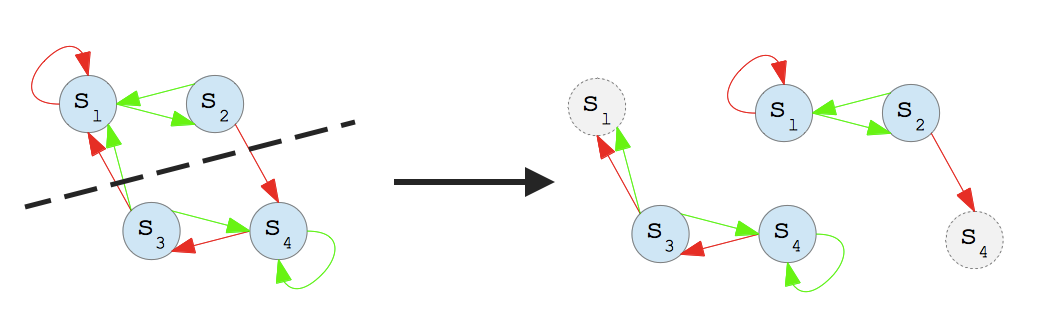
\includegraphics[scale=0.3]{partition.png}  	
  	\end{center}
  \end{frame}
  \begin{frame}
		\frametitle{Rectangular partitioning}
		
		Observation: Biochemical models have rectangular structure with transitions only between adjacent states.
		
		Optimization: Instead of using randomized hash-based partitioning, the state space is partitioned into similarly sized rectangular blocks. This way, we reduce the communication overhead.
		
		\begin{center}
			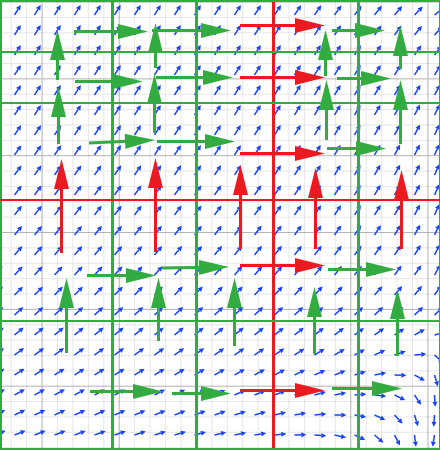
\includegraphics[scale=0.3]{trans.png}		
		\end{center}
  \end{frame}
  \begin{frame}
  	\frametitle{Algorithm}
  	\begin{enumerate}
  		\item Based on distributed CTL model checking algorithm.
  		\item Uses coloured model checking heuristic to reduce runtime for big number of parameters.
  		\item Heuristic is based on two assumptions:
  		\begin{enumerate}
	  		\item Operations on parameter sets are cheaper than state space traversal.
  			\item Small change in parameter leads to small change in transition system.  		
  		\end{enumerate}
  		\item We combine all possible transition systems into one and mark the transitions with parameter values for which they are valid.
  		\item This way, we reduce the number of required traversals significantly, since part of the traversal can be shared by multiple parameters. 	
  	\end{enumerate}
  \end{frame}
  \begin{frame}
  		\frametitle{Example}
  		\begin{center}
  			\includegraphics[scale=0.5]<1-1>{until_first.png}
  			\includegraphics[scale=0.5]<2-2>{until_second.png}
  			\includegraphics[scale=0.5]<3-3>{until_third.png}
  			\includegraphics[scale=0.5]<4-4>{until_fourth.png}  			  			  			
  		\end{center}
  \end{frame}
  \begin{frame}
  	\frametitle{Merge Message Buffer}
  	Observation: Number of messages can grow large when parameter space gets fragmented.
  	
  	Solution: Representing message buffer as an iterable hash table. Two messages with same destination state can be merged into one.  	
  	
  	\begin{center}
	  	\includegraphics[width=\linewidth, keepaspectratio]<1-1>{merge_1.png}  	
	  	\includegraphics[width=\linewidth, keepaspectratio]<2-2>{merge_2.png}  	
	  	\includegraphics[width=\linewidth, keepaspectratio]<3->{merge_3.png}	
  	\end{center}
  \end{frame}
  \begin{frame}
  	\frametitle{Tool Architecture}
  	\begin{center}
		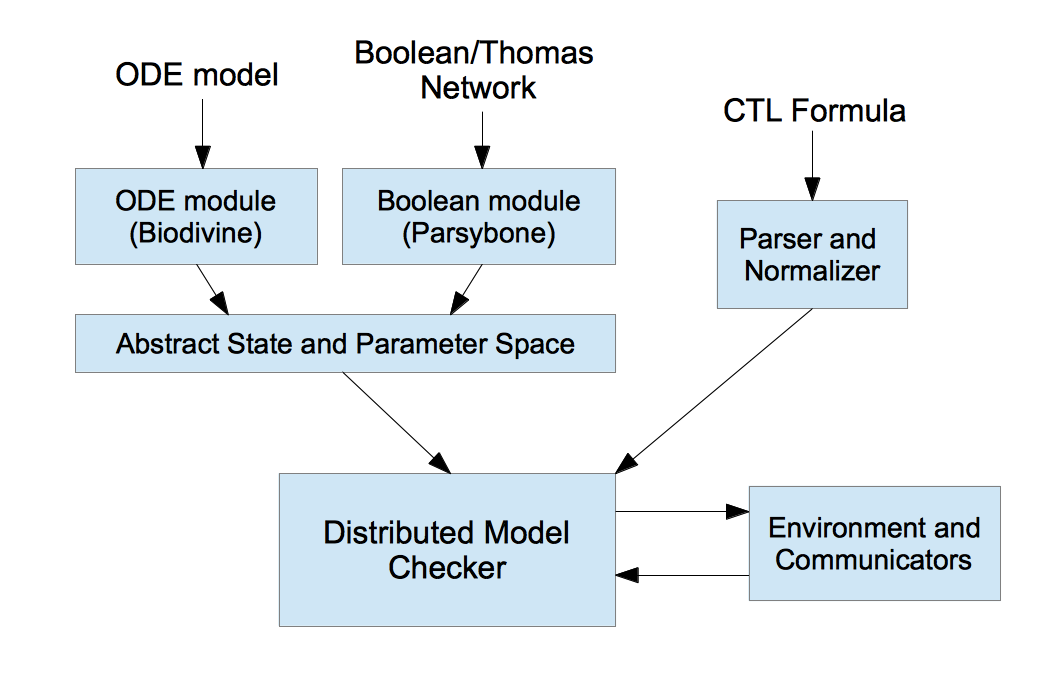
\includegraphics[scale=.55]{architecture.png}  	
  	\end{center}
  \end{frame}
  \begin{frame}
  	\frametitle{Scalability}
  	Testing reachability on enzyme-substrate reversible catalytic reaction
  	\begin{center}
	 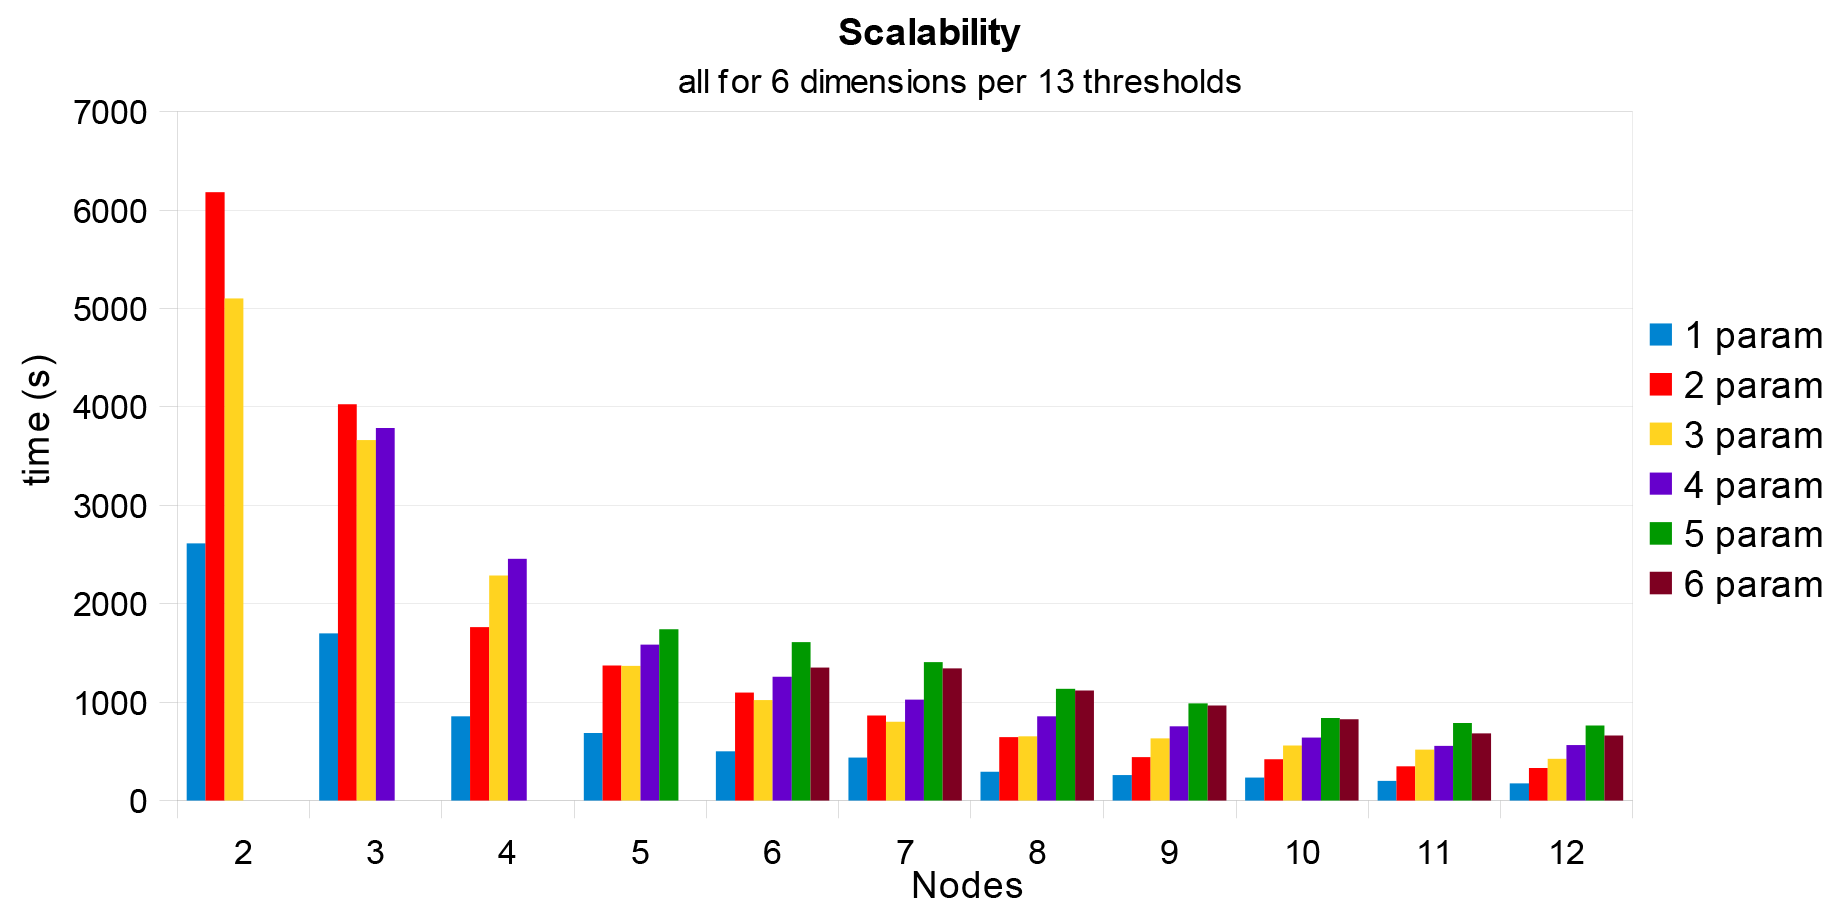
\includegraphics[scale=0.18]{time_series_plot.png}  	
  	\end{center}
  \end{frame}
  \begin{frame}
  	\frametitle{Case Study}
  	\vspace{-4em}
  	Investigating bistability of a well known two gene regulatory network. 
  	\newline\newline\newline\newline\newline
	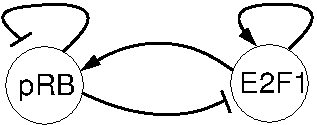
\includegraphics[scale=.63]{gs1net.pdf}
  	\begin{wrapfigure}{r}{0.68\textwidth}
  		\vspace{-11em}
	  \begin{center}
   		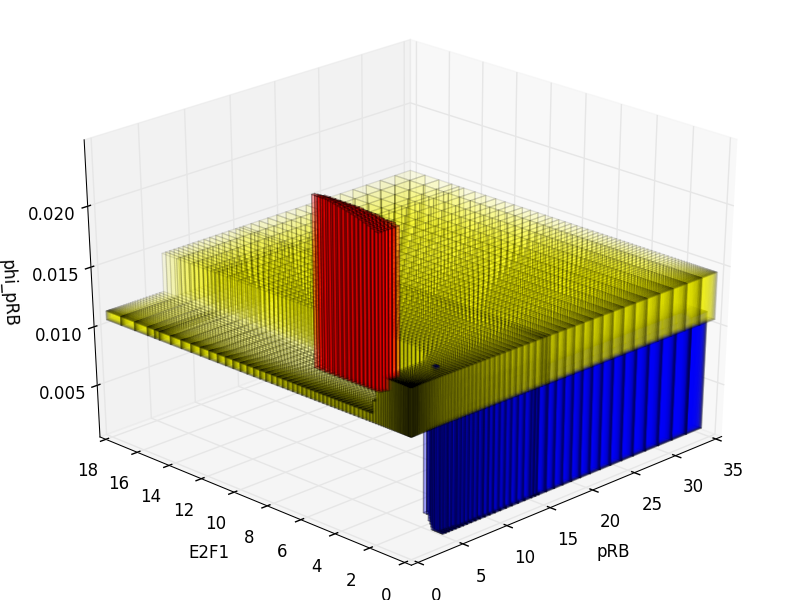
\includegraphics[scale=.43]{3d.png}
	  \end{center}
	\end{wrapfigure}
  \end{frame}
  \begin{frame}
	\begin{center}
		Question Time
	\end{center}
  \end{frame}
% etc
\end{document}